%%%%%%%%%%%%%%%%%%%%%%%%%%%%%%%%%%%%%%%%%%%%%%%%%%%%%%%%%%%%%%%%%%%%%%%%%%%%%%%%
%% Plantilla de memoria en LaTeX para la ETSIT - Universidad Rey Juan Carlos
%%
%% Por Gregorio Robles <grex arroba gsyc.urjc.es>
%%     Grupo de Sistemas y Comunicaciones
%%     Escuela Técnica Superior de Ingenieros de Telecomunicación
%%     Universidad Rey Juan Carlos
%% (muchas ideas tomadas de Internet, colegas del GSyC, antiguos alumnos...
%%  etc. Muchas gracias a todos)
%%
%% La última versión de esta plantilla está siempre disponible en:
%%     https://github.com/gregoriorobles/plantilla-memoria
%%
%% Para obtener PDF, ejecuta en la shell:
%%   make
%% (las imágenes deben ir en PNG o JPG)

%%%%%%%%%%%%%%%%%%%%%%%%%%%%%%%%%%%%%%%%%%%%%%%%%%%%%%%%%%%%%%%%%%%%%%%%%%%%%%%%

\documentclass[a4paper, 12pt]{book}
%\usepackage[T1]{fontenc}

\usepackage[a4paper, left=2.5cm, right=2.5cm, top=3cm, bottom=3cm]{geometry}
\usepackage{times}
\usepackage[utf8]{inputenc}
\usepackage[spanish]{babel} % Comenta esta línea si tu memoria es en inglés
\usepackage{url}
%\usepackage[dvipdfm]{graphicx}
\usepackage{graphicx}
\usepackage{float}  %% H para posicionar figuras
\usepackage[nottoc, notlot, notlof, notindex]{tocbibind} %% Opciones de índice
\usepackage{latexsym}  %% Logo LaTeX

\title{Virtual reality editor for virtual reality scenes}
\author{Julian A. Perez Muñoz}

\renewcommand{\baselinestretch}{1.5}  %% Interlineado

\begin{document}
\chapter{Estado del arte y tecnologías utilizadas} % título del capítulo (se muestra)
\label{chap:objetivos} % identificador del capítulo (no se muestra, es para poder referenciarlo)
\section{WebGL} % título de sección (se muestra)
\label{sec:WebGl}
WebGL~\cite{webGl} es una tecnología creada por Vladimir Vukicevic \footnote{\url{https://en.wikipedia.org/wiki/Vladimir_Vukićević}}, su trabajo comienza con la creación de un prototipo de OpenGL~\cite{openGL} para el elemento canvas de HTML, llamado Canvas 3D. 

Esta API\footnote{\url{https://es.wikipedia.org/wiki/Interfaz_de_programación_de_aplicacione}} de gráficos 3D basada en OpenGL permite a los navegadores modernos renderizar escenas 3D de una manera estandar y eficiente. Esta idea abrió un universo de posibilidades en las web basadas en entornos 3D como son los videojuegos, visualización científica o imagenes médicas. 

Estaba originalmente basado en OpenGL ES 2.0, especificación creada para el iPhone y iPad, a medida que esta se iba desarollando, su objetivo fue la usabilidad en disitintos sistemas operativos y dispositivos. Utiliza el elemento canvas ya que es una evolución del Canvas 3D y se accede a este mediante el DOM. \footnote{\url{https://en.wikipedia.org/wiki/Document_Object_Model}}

Los programas WebGL estan escritos en en JavaScript y en Shading language, un lenguaje similar a C, C++. Por último, esta tecnología fue diseñada y es mantenida por el grupo, non-profit Khronos Group.

\section{WebXR} % título de sección (se muestra)
\label{sec:WebXR}
Sobre esta tecnlogía, WebXR~\cite{webXR}, quizá no hayas escuchado hablar, pero si de WebVR, ya que antes del 2020 ese era su nombre. Con el objetivo de acceder a las principales capacidades de los dispositivos tanto de realidad aumentada (AR), de realidad virtual(VR) como de realidad mixta, el nombre VR, carecía de sentido ya que en cuanto a los dispositivos que englobaba, las siglas VR se quedaban cortas. Otra diferencia importante sobre esta evolución, es el soporte de controladores de entradas basado en la API gamepad\footnote{\url{https://developer.mozilla.org/en-US/docs/Web/API/Gamepad_API/Using_the_Gamepad_API}}.

Otra pregunta muy común sobre esta tecnología es, ¿Tienen la misma relación OpenXR\footnote{\url{https://www.khronos.org/openxr/}}-WebXR que OpenGL-WebGl? la respuesta es no, ya que ambas son distintas API desarrolladas por distintas organismos. 

Para poder entender mejor que es WebXR, debemos tener claro, que hace y que no. WebXR permite manejar el proceso de renderización de las vistas que simulan la experiencia 3D y proporciona los datos necesarios para actualizar las imagenes mostradas al usuario. Debemos tener claro que no es una tecnología de renderizado, WebGL te ayuda con esto.

Los principales casos de uso de esta API son desde la visualización de objetos/datos hasta experiencias artísticas. 

\section{Three.js} % título de sección (se muestra)
\label{sec:Three}
Three.js\footnote{\url{https://threejs.org}} es una biblioteca y una API escrita en JavaScript cuyo objetivo principal es crear y visualizar figuras en 3D. Esta tecnlogía usa WebGL y es capaz de mostrar las figuras en el navegador. Esta biblioteca tiene diversas características como son efectos, escenas, animaciones, materiales o sombreados. También soporta la realidad aumentada o virtual apoyandose en WebXR.

Three.js fue creada por Ricardo Cabello en 2010 y hoy en día está alojado en GitHub.

A continuación puedes ver un ejemplo de un escena creada con three.js
\begin{figure}
  \centering
  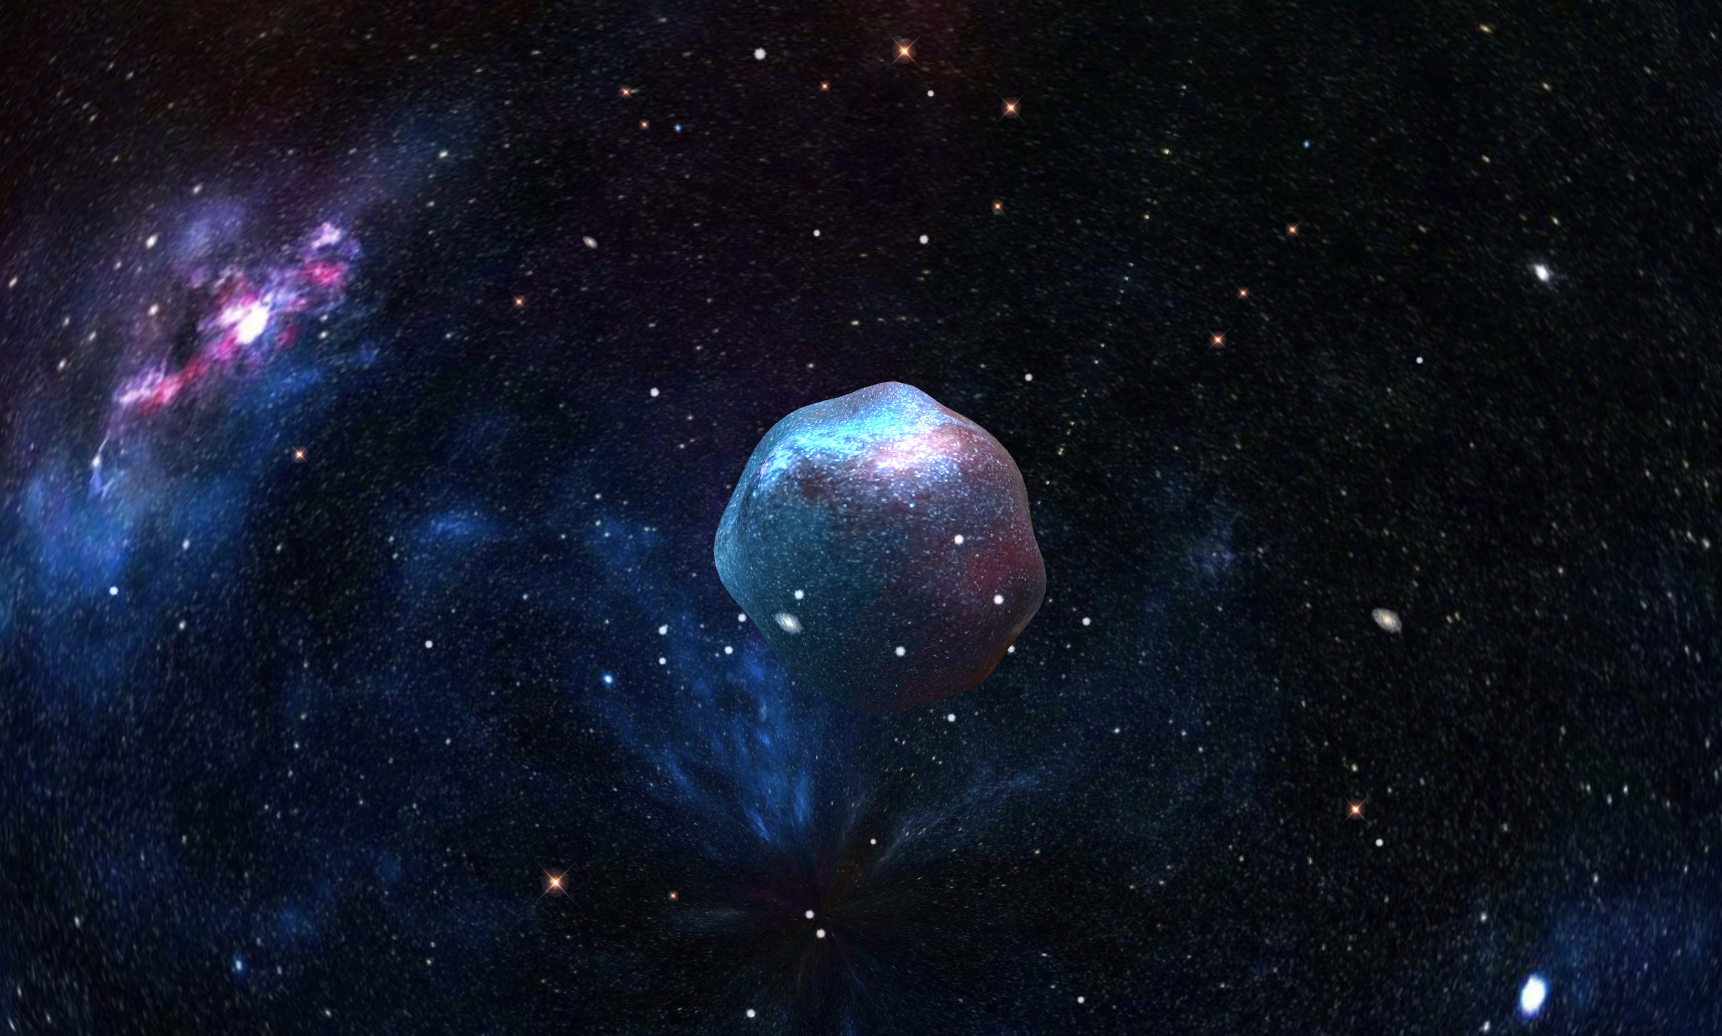
\includegraphics[width=9cm, keepaspectratio]{img/threejs.png}
  \caption{Escena creada con three.js}\label{fig:three}
\end{figure}


\section{HTML5} % título de sección (se muestra)
\label{sec:HTML5}
HTML es uno de lo pilares fundamentales de este proyecto ya que es uno de las tecnologías mas usadas para la creación de este proyecto.

HTML~\cite{HTML} es un lenguaje de marcado utilizado en el desarrollo del contenido web. Suele estar acompañado por otras tecnologías que la complementan, en cuanto a apariencia, CSS, no muy utilizada en este proyecto y en cuanto a funcionalidad, JavaScript, muy utilizada en este trabajo.

Una de las características de HTML es la utilización de marcas para etiquetar los distintos elementos del documento para luego mostrarlo en la web. Algunas de las etiquetas son: \begin{verbatim}<head>, <ul>, <p>, <span>.\end{verbatim} 

Estas etiquetas permiten al elemento tener una gran versatiliad, estructura lógica y facilidad a la hora de entenderlo. Dentro de estas podemos encontrar los atributos\footnote{\url{https://es.wikipedia.org/wiki/Atributo_HTM}} que son utilizados para controlar el comportamiento de dicha equiqueta.

Un ejemplo básico de un documento HTML puede ser el siguiente:

\begin{verbatim}
<!DOCTYPE html>
<html>
  <head>
    <meta charset="utf-8">
    <title>TFG Julian</title>
  </head>
  <body>
    <p>Hola mundo!</p>
  </body>
</html>
\end{verbatim}
Cuando hablamos de HTML es importante destacar el DOM, es la estructura de todos elementos del documento organizados en nodos, el conjunto de todos estos se denomina arbol de nodos. Gracias al DOM y al lenguaje JavaScript podremos acceder a los elementos para un libre utilización de ellos.


\begin{figure}[H]
  \centering
  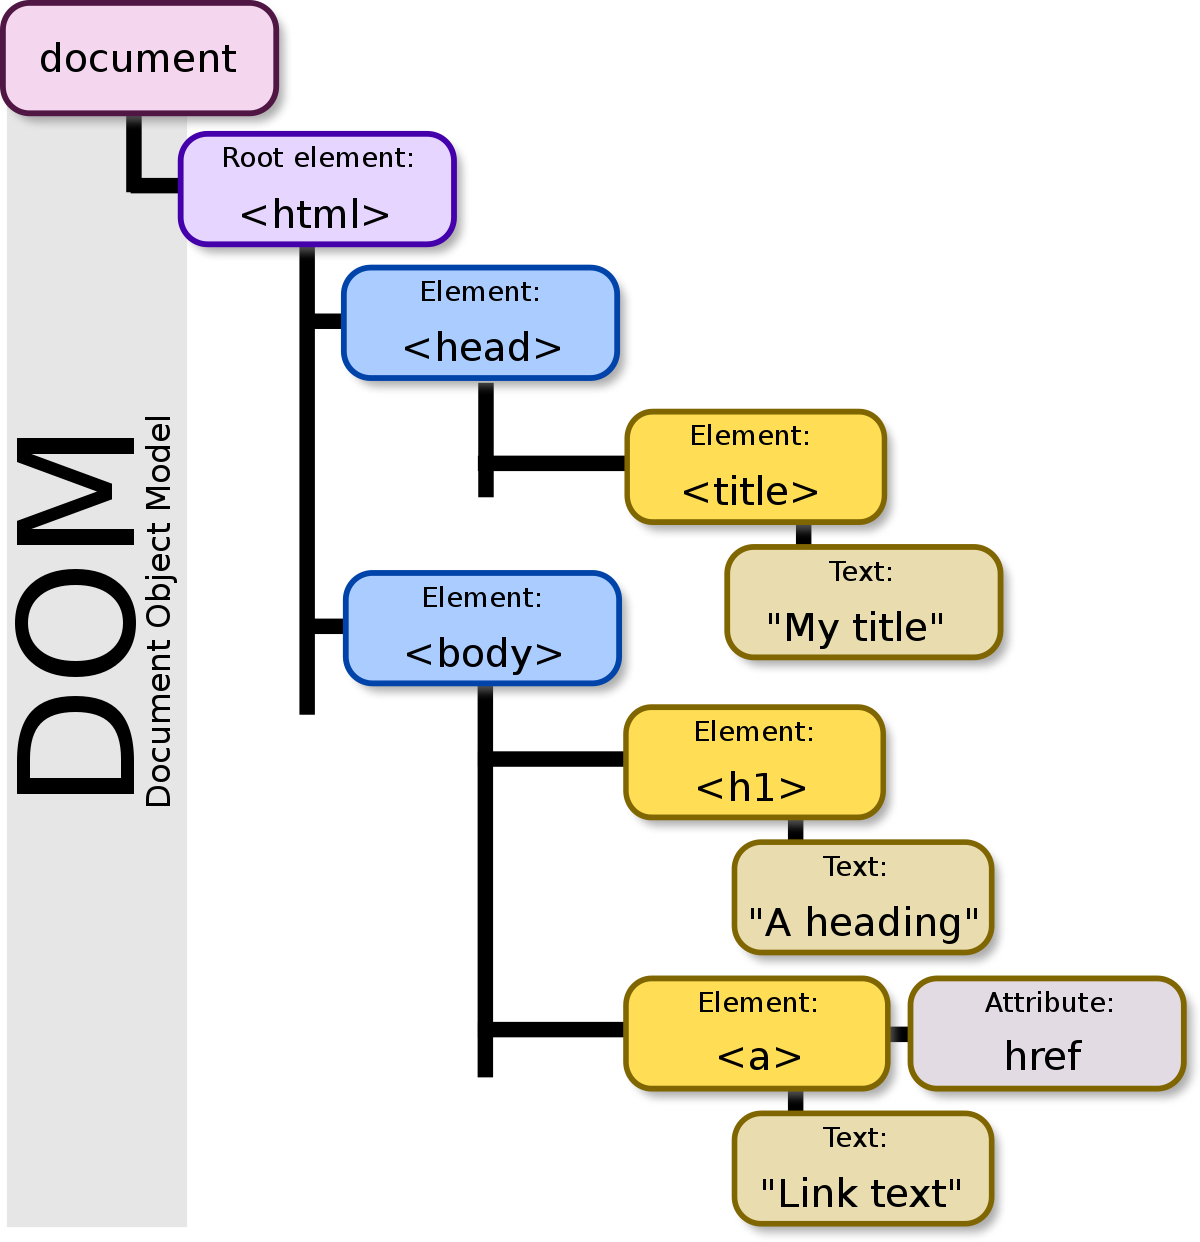
\includegraphics[width=9cm, keepaspectratio]{MemoriaTFG-JulianPerez/img/1200px-DOM-model.svg.png}
  \caption{Visualización gráfica del DOM}\label{html}
\end{figure}


Para terminar, destacar que ahora mismo HTML se ecuentra en su versión HTML5, publicada en 2014, donde se añadieron varias nuevas funcionalidades como la inclusión de nuevas etiquetas o la compatibilidad con varias APIS con Canvas o WebGL.
\section{JavaScript} % título de sección (se muestra)
\label{sec:JavaScript}

JavaScript(JS)~\cite{eloquent} es el lenguaje de programación que se complementa con el lenguaje anteriormente explicado, HTML. JS se suele utlizar para controlar comportamientos de la página web.

Para ampliar información sobre este, podemos decir que JavaScript es un lenguaje que permite la construcción de objetos basada en prototipos\footnote{\url{https://es.wikipedia.org/wiki/Programación_basada_en_prototipos}}, esto ayuda al programador ha crear objetos no mediante el uso de  instancias de clases sino mediante la clonación de objetos. La sintaxis de Javascript con la intención de no complicar mucho este, es muy parecida a otros lenguajes como Java y C++.

Centrandonos en las funcionalidades que ofrece este lenguaje, Javascript nos permite crear los comportamientos de los distintos elementos  HTML mediante el acceso al DOM, A continuación puedes ver un pequeño ejemplo de como realizar un hola mundo en JavaScript:


\begin{verbatim}
 <script>
  document.write("Hola Mundo");
</script>   
\end{verbatim}

Gracias a este lenguaje, puedes crear contenido de actualización dinámica con la creación de eventos, controlar multimedia o animar imágenes, por lo que HTML deja de ser un lenguaje estático.

JavaScript se utiliza principalmente del lado del cliente como parte del navegador web. Si hablamos del lado del servidor podemos hablar de Node.js\footnote{\url{https://nodejs.org/es/}}, se trata de un entorno  en tiempo de ejecucion basado en JS



\section{A-Frame} % título de sección (se muestra)
\label{sec:A-Frame}

A-frame~\cite{a} es la tecnología más importante de este proyecto, ya que es la base fundamental de este. A-frame es un framework creado para la construcción de experiencias en realidad virtual, basado en HTML, por lo que como hemos dicho antes, es un leguaje bastane sencillo e intuitivo. Una de las caracteristicas claves de A-frame es el framwork entidad-componente para three.js.

Esta tecnología fue desarrollada por el equipo de mozilla VR durante 2015. El objetivo principal de estos era permitir crear dichas escenas directamente en HTML sin conocer WebGL. A parte de esta, también usa otras tecnologías anteriormente explicadas como son WebXR y JavaScript.

Un ejemplo de creación de figuras en A-frame mediante HTML puede ser el siguiente:\begin{verbatim}
<html>
  <head>
    <script src="https://aframe.io/releases/1.2.0/aframe.min.js"></script>
  </head>
  <body>
    <a-scene>
      <a-box position="-1 0.5 -3" rotation="0 45 0" color="#4CC3D9"></a-box>
      <a-sphere position="0 1.25 -5" radius="1.25" color="#EF2D5E"></a-sphere>
      <a-cylinder position="1 0.75 -3" radius="0.5" height="1.5" color="#FFC65D"></a-cylinder>
      <a-plane position="0 0 -4" rotation="-90 0 0" width="4" height="4" color="#7BC8A4"></a-plane>
      <a-sky color="#ECECEC"></a-sky>
    </a-scene>
  </body>
</html>
\end{verbatim}

El resultado en la página web de este codigo, es el siguiente:

\begin{figure}[H]
  \centering
  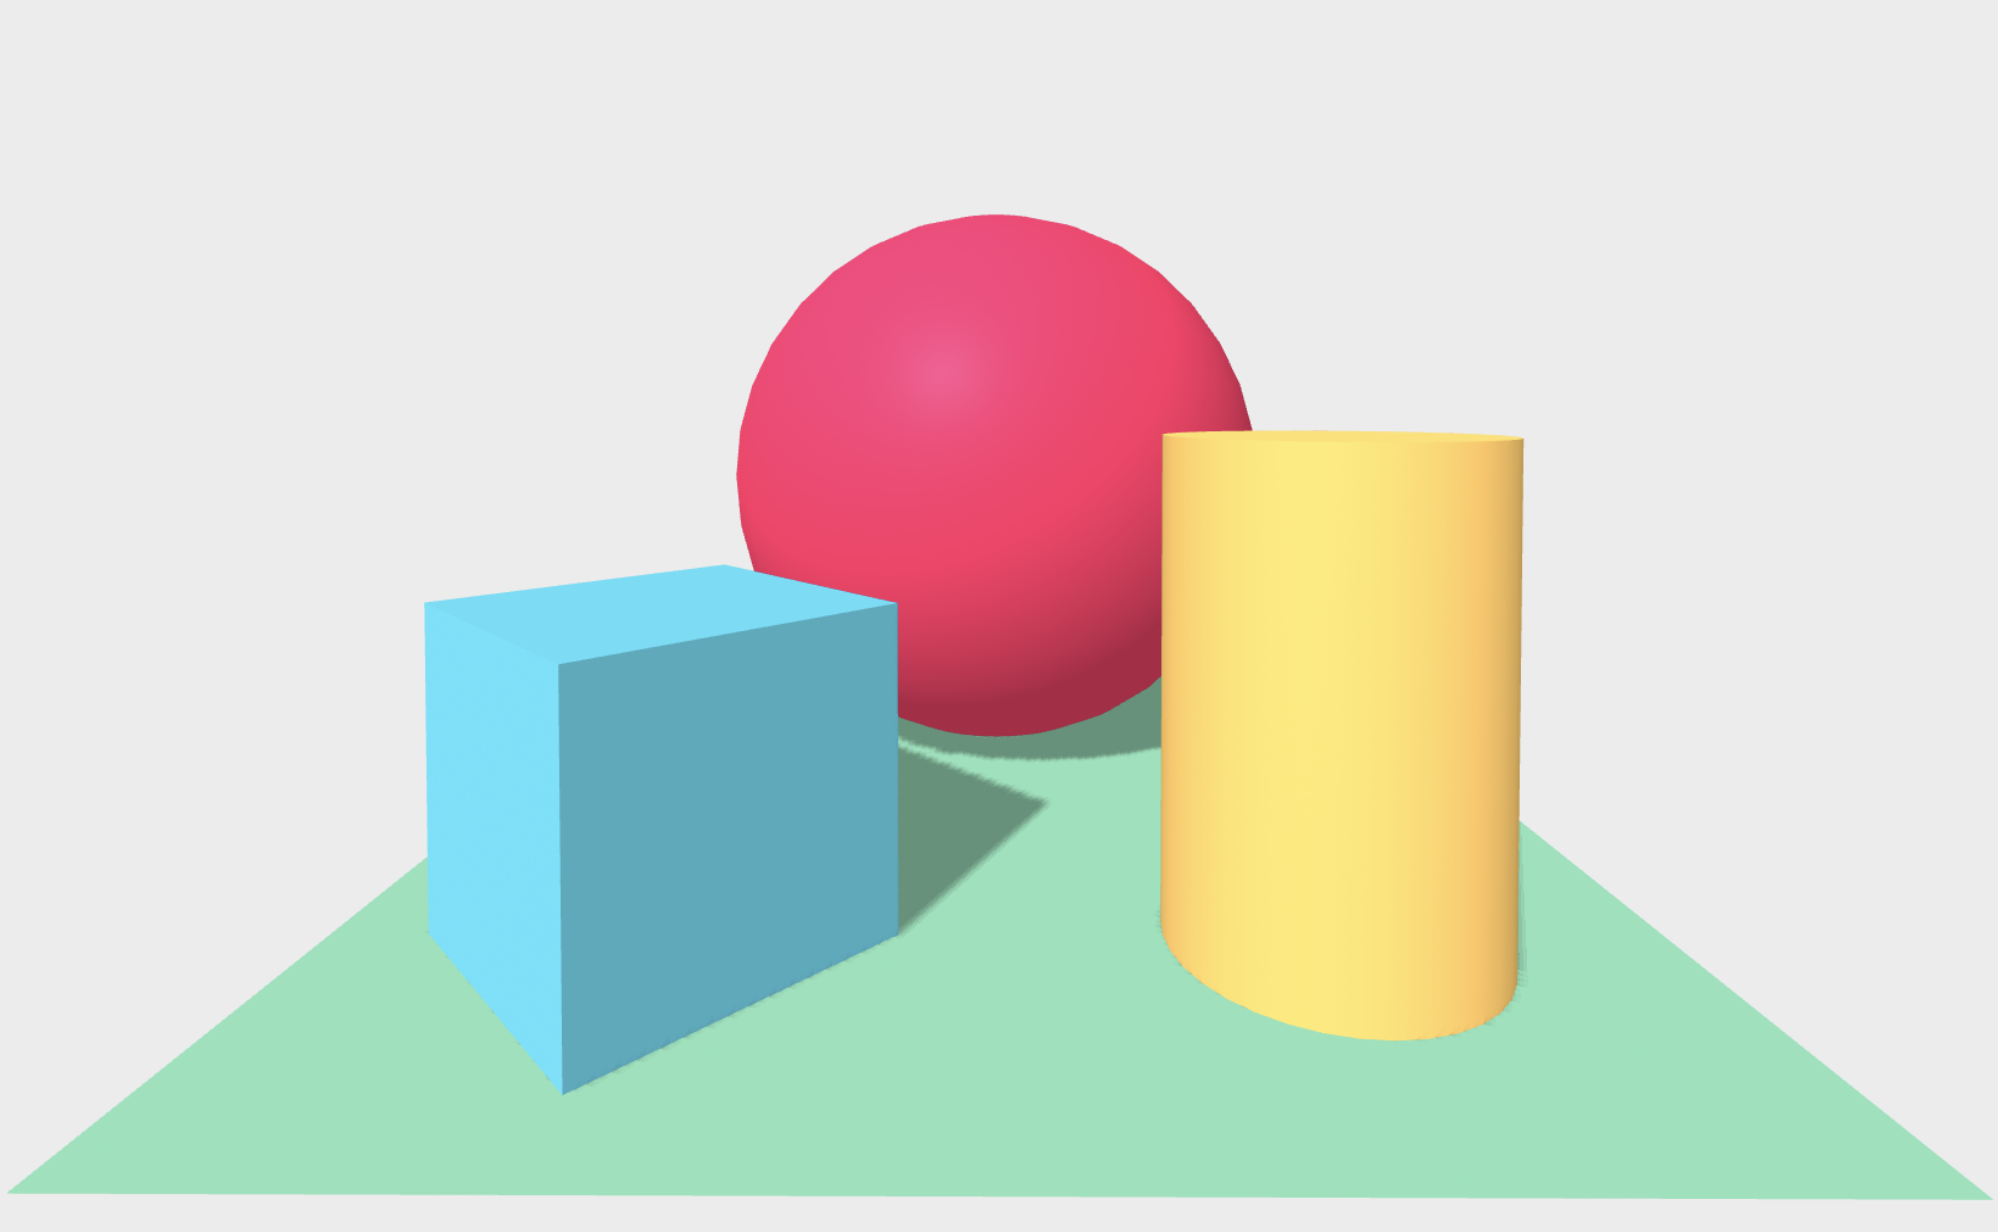
\includegraphics[width=12cm, keepaspectratio]{MemoriaTFG-JulianPerez/img/aframe.png}
  \caption{Escena básica A-Frame}\label{aframe}
\end{figure}

Explicando un poco mas sobre el codigo del escenario de ejemplo, podemos destacar: 

\begin{itemize}
    \item La inclusion de las dependencias de Aframe en el elemento Head, esto nos permite usar todos los elementos de esta tecnología.
    \item La creacion de las diferentes figuras mediante sus respectivas etiquetas.
    \item Modificación de ciertos aspectos de las figturas mediante los atributos.
\end{itemize}

Profundizando un poco más sobre la relación entidad-componente, Una entidad es el objeto en sí creado mediante HTML y el componente es el corportamiento que le podemos asginar a dicha figura, estos se realiza en el JavaScript. 

Estos componentes siguen una estructura estandarizada, algunos son elementos de dicha estructura son: schema, propiedas del componente, init, parte del componente que se ejectuta al iniciar el componente. La manera correcta de incluir un componente a la escena es añadirselo al elemento como si de un atributo se tratara.

 
\section{Github} % título de sección (se muestra)
\label{sec:GitHub}
GitHub~\cite{GITHUB} es una platafroma de almacenamiento y administración  de software, Este sistema está basado en el control de versiones \footnote{\url{https://es.wikipedia.org/wiki/Control_de_versiones}} y en Git \footnote{\url{https://git-scm.com}}.

Gracias al control de versiones, el desarrollador puede administrar y llevar un registro de cualquier modificación sobre el proyecto. Este sistema permite al desarrollador trabajar de una forma segura mediante las ramas. Las ramas te permiten duplicar el codigo fuente, donde puede hacer cambios sin afectar al proyecto "principal". Puedes fusionar las distintas ramas si lo deseas.

En cuanto a Git, se trata de un sistema de control de versiones, es decir te ayuda a controlar lo anterior explicado mediante el terminal del ordenador.

Tras esto, podemos explicar de una manera mas específica que es Github, este es una interfaz gráfica de Git el cual nos ofrece distintas funcionalidades como pueden ser, la creación de un usuario, la creación de distintos proyectos(repositorios) los cuales modificar desde la propia interfaz web, capacidad de trabajar en repositorios creados por otros desarrolladores mediante un fork\footnote{\url{https://es.wikipedia.org/wiki/Bifurcación_(desarrollo_de_software)}} o la modificación del mismo mediante un pull, creacion de un foro en los que los desarroladores pueden expresar dudas/problemas sobre el proyecto, etc.

Hoy en día según el 87\% de los desarrolladores utilizan GitHub, en mi caso ha sido la plataforma principal en la cual he ido utilizando para el desarrollo del proyecto.


\section{PyCharm} % título de sección (se muestra)
\label{sec:GitHub}
Se trata de un entorno de desarrollo integrado (IDE) que se utiliza para la programación, es un software creado por la compañia JetBrains~\cite{jetbrains}.

Este software es multiplataforma adaptado para Windows, macOS y Linux. Ha sido utilizado para la creación de este proyecto y por eso es una parte fundamental de esto.

Tiene infinidad de ventajas entre las que están:

\begin{itemize}
    \item Asistencia y análisis de codificación, con ayuda a la finalización del codigo, sintaxis y resaltado de errores.
    \item Navegación entre proyectos y ficheros.
    \item Acceso a la ejecución del codigo en el navegador mediante accesos directos.
\end{itemize}

Pycharm proporciona una API para que los desarrolladores puedan crear distintos plugins y de este modo se pueda crear codigo de manera más facil y eficiente.

\section{Latex} % título de sección (se muestra)
\label{sec:Latex}
LaTeX está basado en Tex\footnote{\url{https://es.wikipedia.org/wiki/TeX}}, programa destinado a la creación de documentos que contienen textos y fórmulas matemáticas. Este programa no es un editor de textos, si no, un procesador de macros.

LaTeX es un conjunto de macros para Text, cuyo objetivo principal es la alta composición tipográfica. Está orientando a la producción y creación de documentos científicos y se ha estandarizado para la creación de los mismos.

Esta tecnología nos presenta diversas ventajas entre las que se encuentran la faciliad de gestionar las referencias, bibliografias, etc, es un sistema multiplataforma, puedes componer fórmulas con calidad de imprenta o la capacidad de exportar el documento a PDF. La creación de dichos documentos puede ser al principio, un poco complicado si no se conoce la herramienta.

Se trata de un softwate libre bajo la licencia LPPL\footnote{\url{https://es.wikipedia.org/wiki/LaTeX_Project_Public_License}} 

Este sistema ha sido fundamental a la hora de crear este proyecto ya que esta memoria esta creada utilizando LaTeX.

\section{Gltfs} % título de sección (se muestra)
\label{sec:Gltfs}
Este formato de archivo tiene como objetivo principal escenas y modelos en 3D y esta basado en el foramto de texto sencillo para el intercambio de datos, JSON. Porpularmente se le describe como como el JPEG en 3D.

Este formato esta creado para una eficiente distribución de objetos y escenas en 3D, disminuyendo el tiempo de procesameinto en ejecución. Este formato se puede usar en aplicaciones que usan la tecnología anteriormente explicada, WebGl.

Es importante explicar este formato, ya que la aplicación que he creado te permite el manejo y  modificación de este formato en la aplicación.

\section{Otros} % título de sección (se muestra)
\label{sec:Otros}
En esta sección es importante destacar otros editores que trabajar en VR como son Blender, centrado en aspectos como la renderización, creación de gráficos en 3D o Unity centrado en creación del motror gráfico en videojuegos. Ya que mi proyecto es un pequeño paso para la creación de un gran editor.

Existen otros editores como son, OpenCat o AutoCat.
\end{document}